\documentclass[a4paper, 12pt]{article}
\usepackage{amsmath}
\usepackage[utf8]{inputenc}
\usepackage{graphicx}
\usepackage{parskip}
\usepackage{tikz}
\usepackage{tkz-graph}
\usepackage{tikzscale}
\usetikzlibrary{arrows}

\begin{document}

\title{\vspace{-6em}\textbf{Homework 2}\\ \Large Information Theory for Complex Systems \vspace{-1em}}
\author{}
\date{\vspace{-3.2em}}

\maketitle

\subsection*{a)}
The automata is desterministic everywhere except for the middle node. If one traverses the edge which arcs backwards, the sequence is always 011. And if the edge to the right is chosen, the following sequence is always 001. Therefore we can construct and optimal code using the two symbols $a = 011$ and $b = 001$ transforming the automata into an equivalent one presented in figure \ref{fig:code}.

\begin{figure}[ht]
\begin{center}
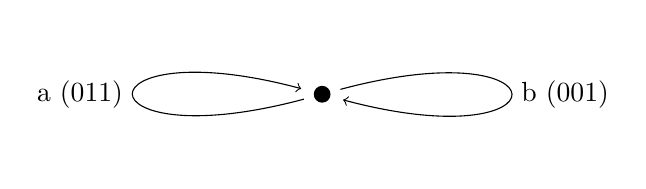
\begin{tikzpicture}[main node/.style={circle,draw,fill,inner sep=2pt,outer sep=4pt},scale=6]
    \node[main node] (1) {};
    \path
        (1) edge [loop left] node {a (011)} (1)
            edge [loop right] node {b (001)} (1);
\end{tikzpicture}
    \caption{Optimal code representation of the finitite state automata. Both transitions are equally likely.}
    \label{fig:code}
\end{center}

\end{figure}

This compressed automata generates a random sequence of "coin flips" between $a$ and $b$. Since it is completely uniformly random, binary sequence the entropy per symbol is $s_{a,b} = 1\,$bit. The original sequence of 1's and 0's contains three symbol per $a$ or $b$ so the resulting entropy per symbol is $s = 1/3\,$bit.

\subsection*{b)}
The longest correlation needed in order to determine the probability distribution for the following symbols is 3. Every sequence longer than 3 necessarily contains at least one copy of $a$ or $b$ allowing one to identify where in the automata the current state is located.

\subsection*{c)}
Equation (3.36) gives
\begin{equation}
    \eta = \sum_{m=1}^{\infty} (m-1)k_m.
\end{equation}
As has already been discussed, $k_m = 0,\,\, \forall m > 3$ which leaves us with the task of calculating $k_1, k_2$ and $k_3$. Following (3.18) gives
\begin{equation}
    k_1 = p(0) \log(2p(0)) + p(1) \log(2p(1)) = \frac{1}{2} \log(1) + \frac{1}{2} \log(1) = 0.
\end{equation}
We can then
\begin{equation}
    \begin{split}
        k_2 = p(0) \left[p(0|0) \log \frac{p(0|0)}{p(0)} + p(1|0) \log \frac{p(1|0)}{p(0)}\right] + \\
        p(1) \left[p(0|1) \log \frac{p(0|1)}{p(1)} + p(1|0) \log \frac{p(1|1)}{p(1)}\right] = \\
        \frac{1}{2} \left[ \frac{1}{3} \log \frac{1/3}{1/2} + \frac{2}{3} \log \frac{2/3}{1/2} \right] +
        \frac{1}{2} \left[ \frac{2}{3} \log \frac{2/3}{1/2} + \frac{1}{3} \log \frac{1/3}{1/2} \right] = \\
        \left[ \frac{2}{3} \log \frac{4}{3} + \frac{1}{3} \log \frac{2}{3} \right]  \approx\\
        0.0817...
    \end{split}
\end{equation}

We also have the equation
\begin{equation}
    k_{corr} = S_{max} - s = 1 - \frac{1}{3} \iff k_{corr} = \frac{2}{3} = k_1 + k_2 + k_3
\end{equation}
with all values being known except $k_3$. We find out
\begin{equation}
    k_3 = \frac{2}{3} - 0 - \left[ \frac{2}{3} \log \frac{4}{3} + \frac{1}{3} \log \frac{2}{3} \right] \approx 0.58496.
\end{equation}
Finally reinserting for $\eta$ gives $\eta \approx 1.25162$.

\end{document}
